\paragraph{La classe Frame}

\begin{minipage}
    {\linewidth}
    \centering
    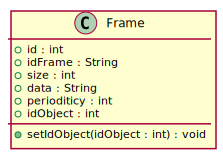
\includegraphics[width=0.80\linewidth]{../schemas/Conception_detaillee/classe_frame.pdf}
    \captionof{figure}{Diagramme de classe de Frame}
\end{minipage}

\subparagraph{Philosophie de conception \newline} 

\medspace

La classe Frame définit les attributs des trames. 

\subparagraph{Description structurelle \newline}

\medspace

\textbf{Attributs :}

\begin{itemize}
    \item \textbf{id : int} --- Identifiant unique et interne à l'application de la trame afin de l'identifier. 
    \item \textbf{idFrame : String} --- Identifant de la trame. 
    \item \textbf{size : int} --- Taille de la trame.
    \item \textbf{data : String} --- Message de la trame. 
    \item \textbf{periodicity : int} --- Périodicité de la trame, la valeur est à 0 lorsque la trame est ponctuelle. 
    \item \textbf{idObject : int} --- Identifiant permettant de lier un objet à la trame. 
\end{itemize}


\textbf{Services offerts :}

\begin{itemize}
    \item \textbf{setIdObject(idObject : int) : void} --- Opération qui permet de définir l'id de l'object (idObject) avec l'objet associé. Cela permet de créer une relation entre les trames et les objets.  
\end{itemize}